\part{Graph&Table}
\subsection{Include graphs}

\begin{frame}
	\frametitle{Include graphs}
	\small
	It's very useful to include graphs in \LaTeX, especially in report and paper writing. Here is a common template of including a single floating graph.
	\begin{command}
		\samplecommand{usepackage}\{graphicx\}\\
		\samplebegin{figure}[\structure{position}]\\
		\qquad\samplecommand{centering}\\
		\qquad\samplecommand{includegraphics}[\structure{options}]\{\structure{file}\}\\
		\qquad\samplecommand{caption}\{\structure{caption}\}\\
		\qquad\samplecommand{label}\{\structure{label}\}\\
		\sampleend{figure}
		\begin{itemize}
			\setlength{\itemsep}{0pt}
			\setlength{\parsep}{0pt}
			\setlength{\parskip}{0pt}
			\item \structure{file} - the filename or relative path of the graph you want to insert, usually placed in the same directory as the tex file
			\item \structure{position} - we usually use \structure{htbp} here, which will be introduced later in this chapter
			\item \structure{options} - the width, height and other options about the graph
			\item \structure{caption} - the caption displayed above/under the graph
			\item \structure{label} - used for references in a document (will be introduced later)
		\end{itemize}
	\end{command}
\end{frame}

\begin{frame}[fragile]
	Usually you need to optimize the size and some other properties of the graph, most of them can be set in \structure{options}. (Only some useful options are listed here)
	\begin{itemize}
		\item \structure{height} - use any \LaTeX\ measuring unit.
		\item \structure{width} - use any \LaTeX\ measuring unit.
		\item \structure{scale} - scale the graph to this proportion
		\item \structure{angle} - rotate the graph in anti-clockwise by this angle 
	\end{itemize}
	\begin{minipage}{0.5\linewidth}
		\begin{example}
			\begin{minted}{latex}
\usepackage{graphicx}
\begin{figure}[htbp]
    \centering
    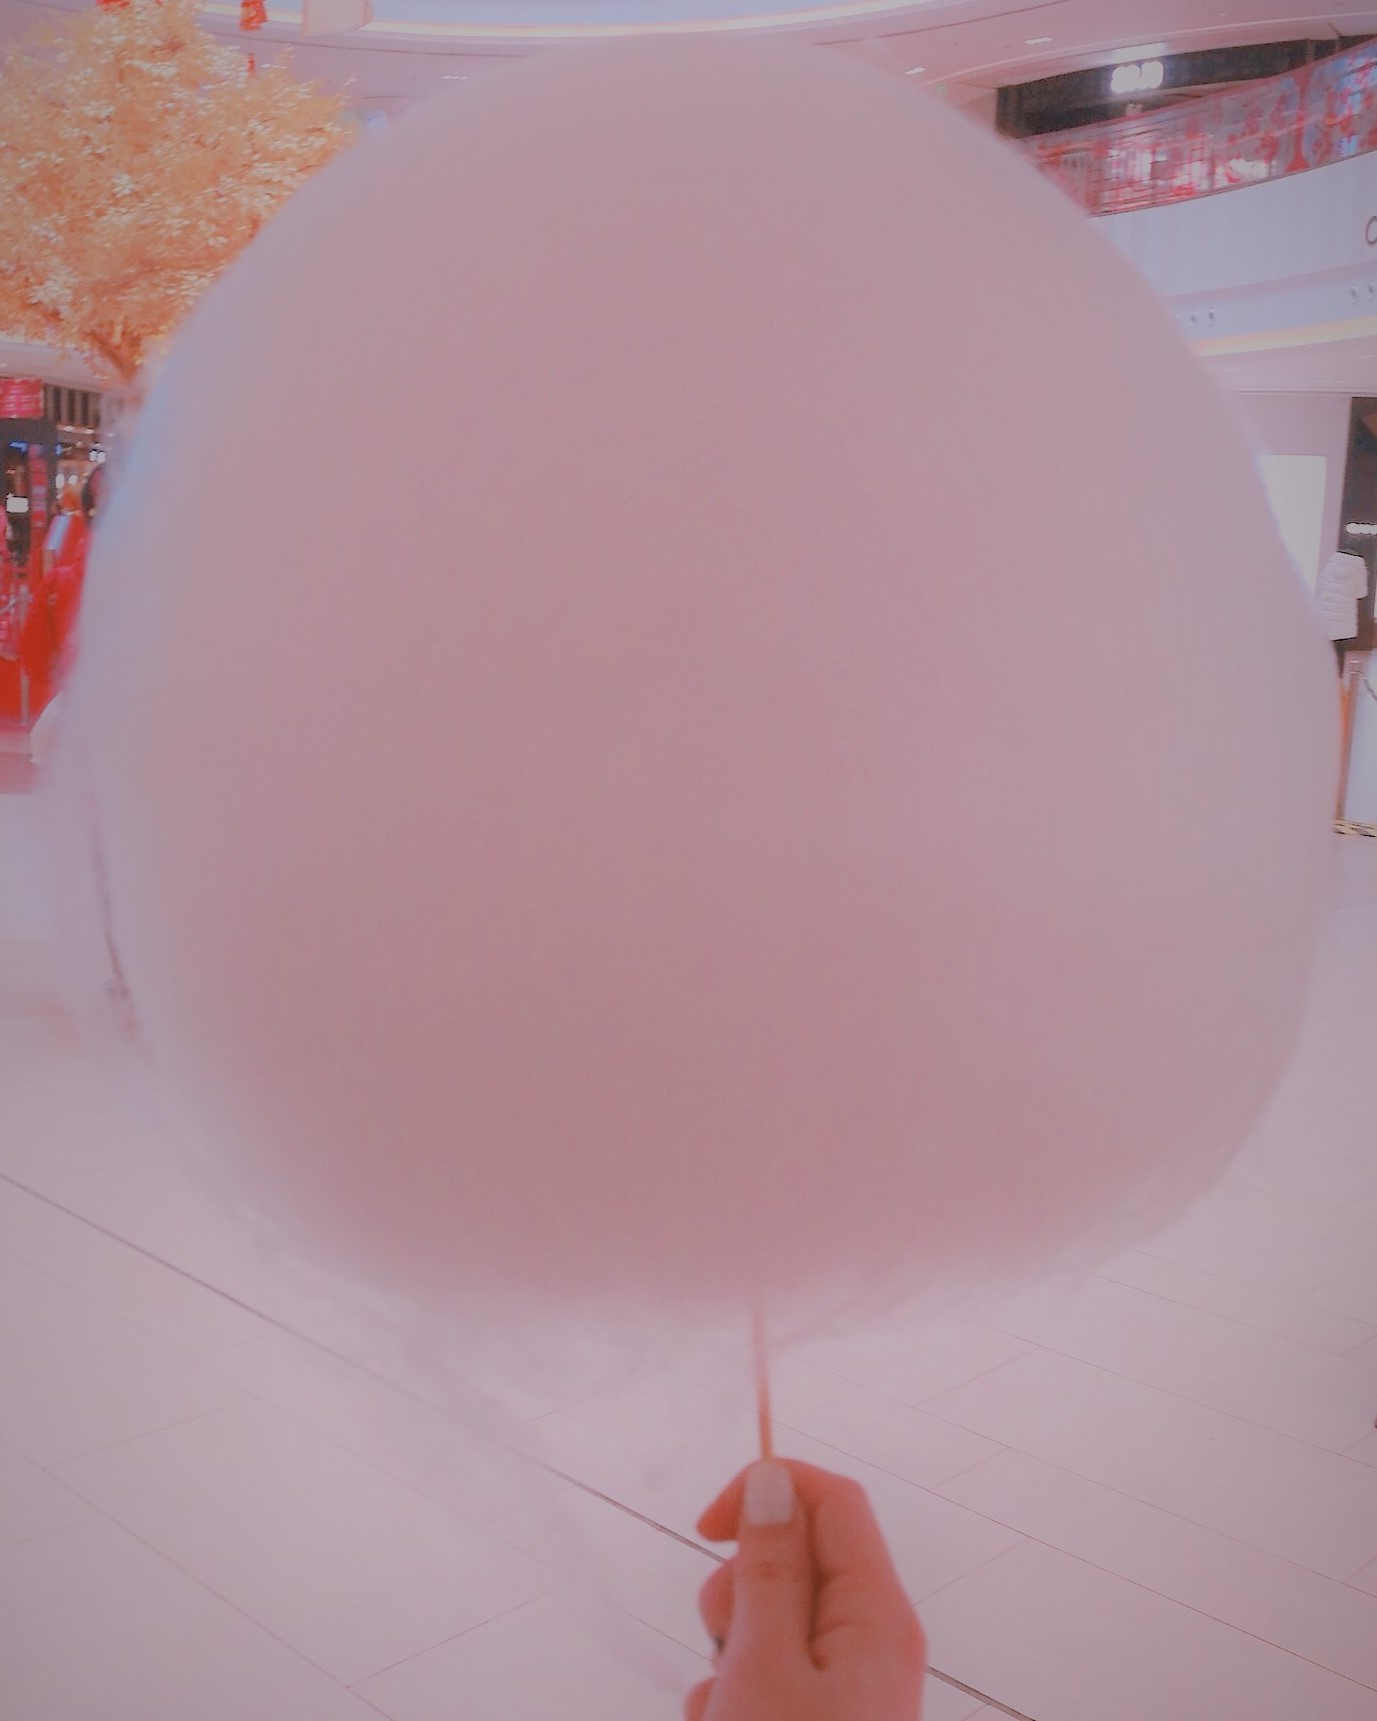
\includegraphics[width=0.5 \linewidth]{sample.jpg}
    \caption{Marshmallow}
    \label{fig-sample}
\end{figure}
			\end{minted}
		\end{example}
	\end{minipage}
	\hfill
	\begin{minipage}{0.45\linewidth}
		\begin{figure}[htbp]
			\centering
			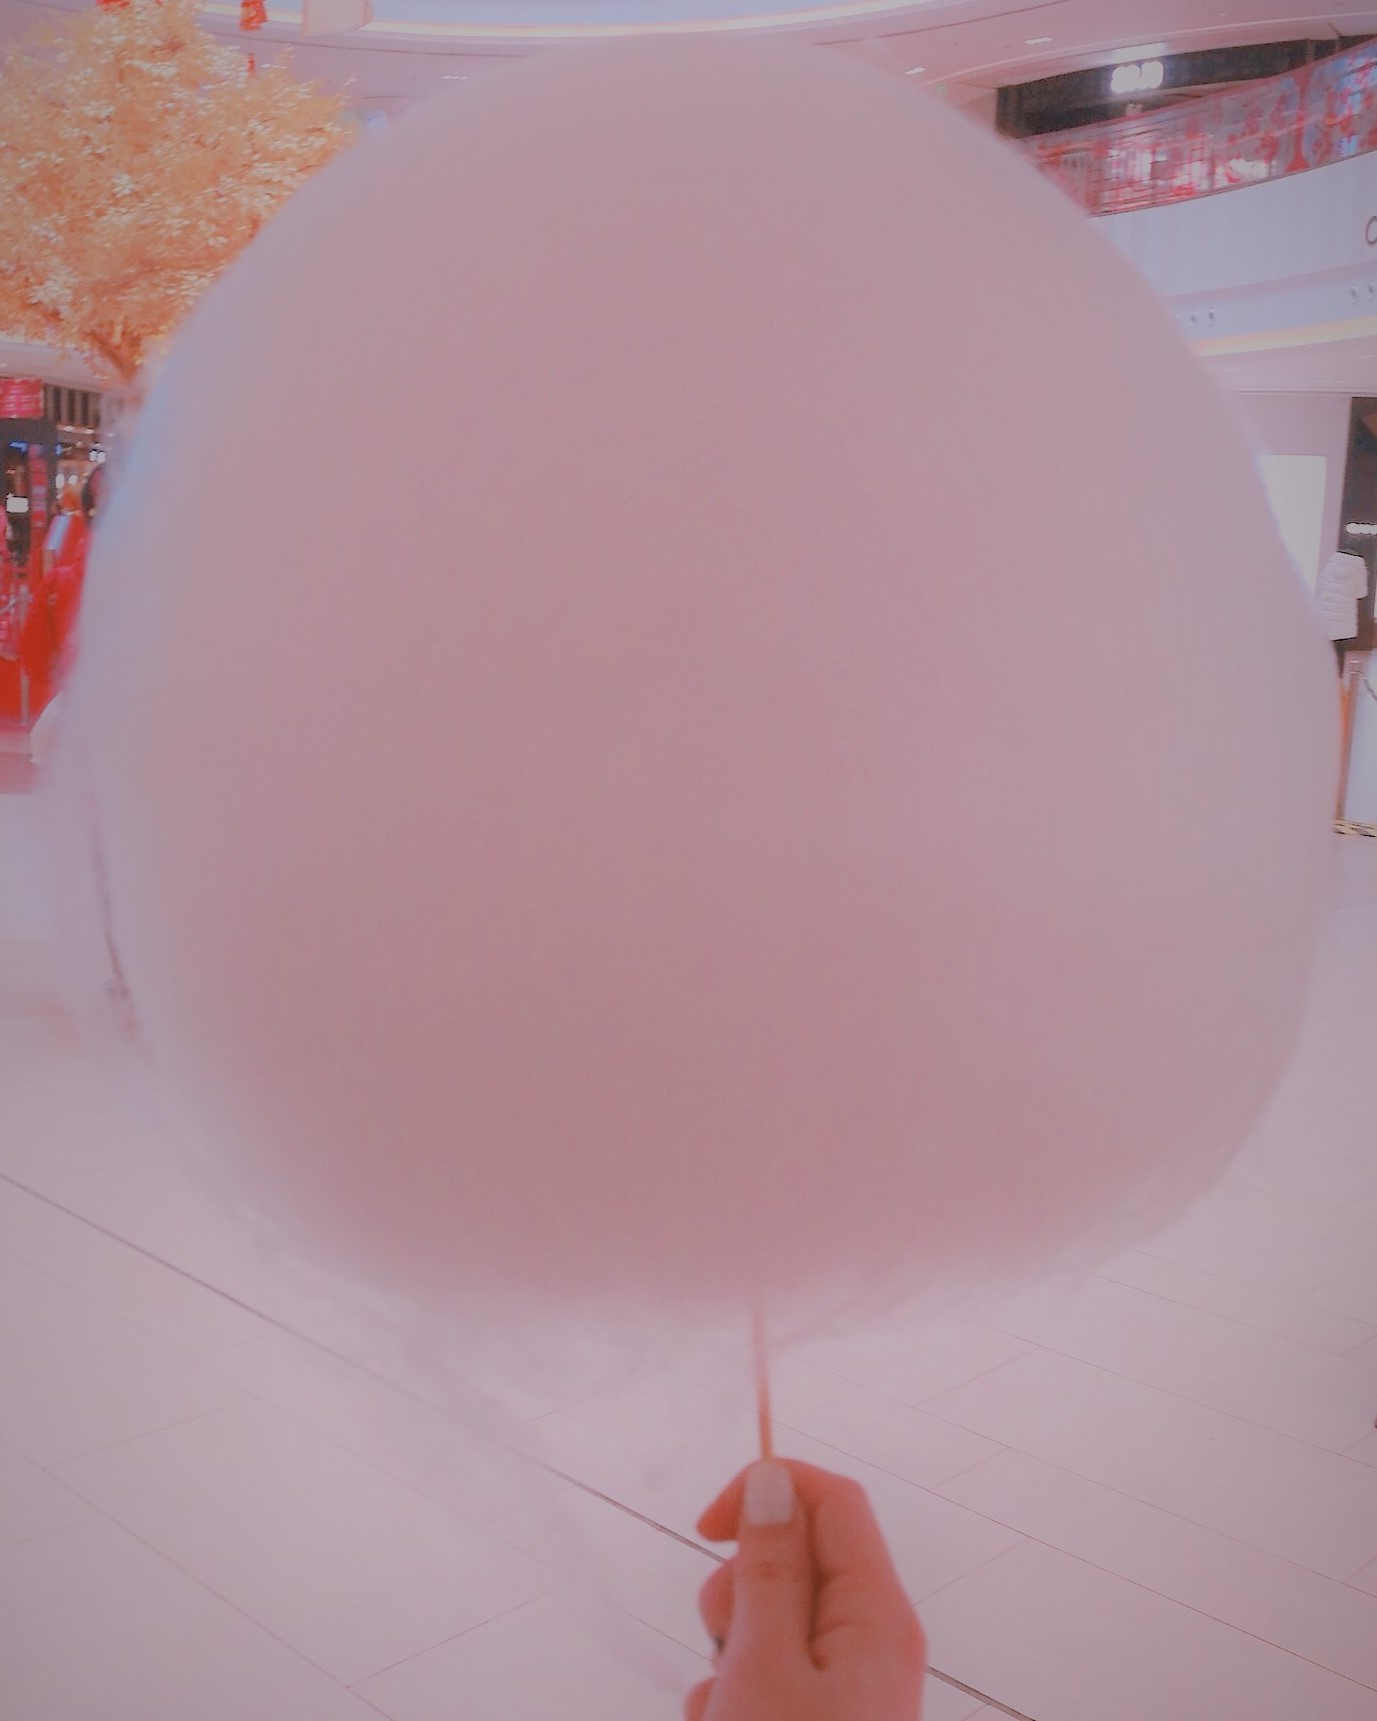
\includegraphics[width=0.5\linewidth,angle=180]{sample.jpg}
			\caption{Marshmallow}
			\label{fig-sample}		
		\end{figure}
	\end{minipage}
\end{frame}

\begin{frame}[fragile]
	\frametitle{Include multiple graphs}
	\structure{Subfigure} package can be used to include a series of graphs.\\
	\begin{minipage}{0.6\linewidth}
		\begin{example}
			\begin{minted}{latex}
\begin{figure}[htbp]
    \centering
    \subfigure[1]{
        
\includegraphics[width=0.4 \linewidth]{sample-1.jpg}
        \label{fig-sample-1}
    }
    \subfigure[2]{
        
\includegraphics[height=0.4 \linewidth]{sample-2.jpg}
        \label{fig-sample-2}
    }
    % more subfigures
    \caption{Marshmallows}
    \label{fig-entire}
\end{figure}
			\end{minted}
		\end{example}
	\end{minipage}
	\hfill
	\begin{minipage}{0.38\linewidth}
		\begin{figure}[htbp]
			\centering
			\subfigure[1]{
				
\includegraphics[width=0.4\linewidth]{sample-1.jpg}
				\label{fig-sample-1}
			}
			\subfigure[2]{
				
\includegraphics[height=0.4\linewidth]{sample-2.jpg}
				\label{fig-sample-2}
			}
			\subfigure[3]{
				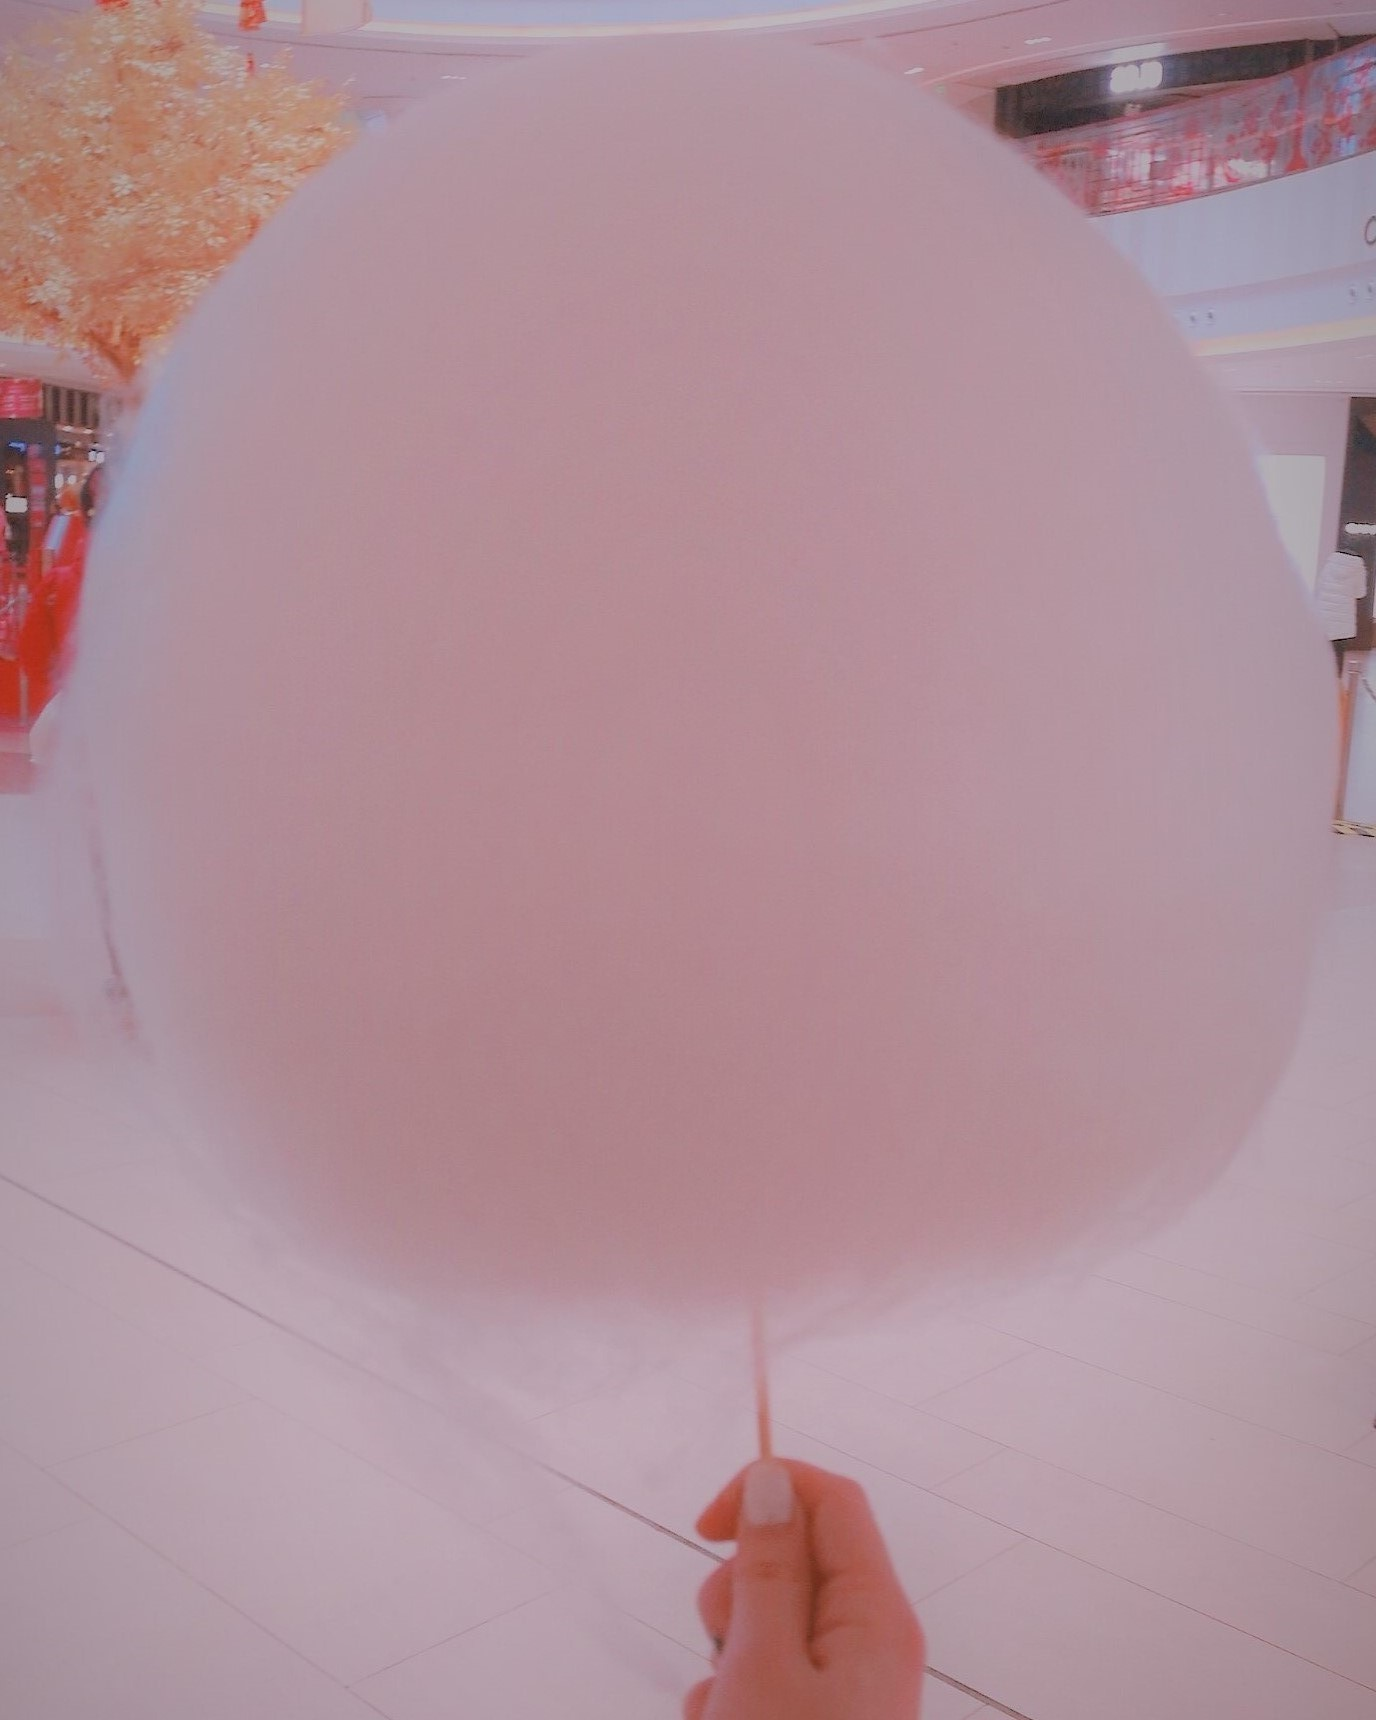
\includegraphics[height=0.4\linewidth]{sample-3.jpg}
				\label{fig-sample-3}
			}
			\subfigure[4]{
				
\includegraphics[width=0.4\linewidth]{sample-4.jpg}
				\label{fig-sample-4}
			}
			\caption{Marshmallows}
			\label{fig-entire}
		\end{figure}
	\end{minipage}
\end{frame}

\subsection{Draw tables}

\begin{frame}[fragile]
	\frametitle{Draw tables}
	Table is another common element in \LaTeX, for example, there is a simple table like this:
    \begin{example}
    	\begin{minted}{latex}
\begin{tabular}{|l|c|r|}
    \hline
    Title 1 & Title 2 & Title 3 \\
    \hline
    1 & 2 &3 \\
    \hline
\end{tabular}
    	\end{minted}
    \end{example}
    \begin{table}[htbp]
    \centering
    \begin{tabular}{|l|c|r|}
        \hline
        Title 1 & Title 2 & Title 3 \\
        \hline
        1 & 2 &3 \\
        \hline
    \end{tabular}
	\end{table}
\end{frame}

\begin{frame}
	\begin{command}
		\samplebegin{tabular}\{\structure{format}\}\\
		\qquad ...\\
		\sampleend{tabular}
	\end{command}
	\structure{format} can be set as follow
	\begin{itemize}
		\item \structure{$|$} - represents a vertical separate line between two columns
		\item \structure{l} - align left in this column
		\item \structure{c} - align center in this column
		\item \structure{r} - align right in this column
	\end{itemize}
	\begin{example}
		\begin{minipage}{0.48\linewidth}
			\centering
			\structure{$|$l$|$l$|$l$|$}\\[0.5em]
        	\begin{tabular}{|l|l|l|}
        		\hline
        		Title 1 & Title 2 & Title 3 \\
        		\hline
        		1 & 2 &3 \\
        		\hline
        	\end{tabular}
		\end{minipage}
		\begin{minipage}{0.48\linewidth}
			\centering
			\structure{$||$c$|$cc$||$}\\[0.5em]
        	\begin{tabular}{||c|cc||}
        		\hline
        		Title 1 & Title 2 & Title 3 \\
        		\hline
        		1 & 2 &3 \\
        		\hline
        	\end{tabular}
		\end{minipage}
    \end{example}	
\end{frame}

\begin{frame}[fragile]
	How to arrange cells in \structure{tabular} environment is very similar to the \structure{align} environment. However, we usually need horizontal lines in tables.
	\begin{command}
		\samplecommand{hline}\quad=\quad\samplecommand{cline}\{1-\structure{max\_col}\}\\
		\samplecommand{cline}\{\structure{start}-\structure{end}\}
	\end{command}
	\begin{minipage}{0.45\linewidth}
		\begin{example}
			\begin{minted}{latex}
\begin{tabular}{c|l|c|r}
    \hline
    \hline
    & Title 1 & Title 2 & Title 3 \\
    \cline{2-4}
    Table & 1 & 2 & 3 \\
    \cline{2-4}
    & 4 & 5 & 6 \\
    \hline
    \hline
\end{tabular}
			\end{minted}		
    	\end{example}
	\end{minipage}
	\hfill
    \begin{minipage}{0.5\linewidth}
    	\ \\[0.5em]
    	\begin{tabular}{c|l|c|r}
        	\hline\hline
        	& Title 1 & Title 2 & Title 3 \\
        	\cline{2-4}
        	Table & 1 & 2 & 3 \\
        	\cline{2-4}
        	& 4 & 5 & 6 \\
        	\hline\hline
        \end{tabular}\\[0.5em]
        Here we draw a table with a multirow, but it only works with multirows of odd row number. A more convenient method of drawing multirows will be introduced.
    \end{minipage}
    
\end{frame}

\begin{frame}
	\frametitle{Multicolumn and Multirow}
	\begin{command}
		\samplecommand{multicolumn}\{\structure{ncols}\}\{\structure{format}\}\{\structure{text}\}\\
		\begin{itemize}
			\item \structure{ncols} - the number of columns to be merged
			\item \structure{format} - the format of the merged column, excluding the left | (eg. c$|$)
			\item \structure{text} - the text in the merged column
		\end{itemize}
		\samplecommand{usepackage}\{multirow\}\\
		\samplecommand{multirow}\{\structure{nrows}\}\{\structure{width}\}[\structure{fixup}]\{\structure{text}\}\\
		\begin{itemize}
			\item \structure{nrows} - the number of rows to be merged
			\item \structure{width} - the width of the merged rows (use \structure{*} for auto)
			\item \structure{fixup} - the vertical position of the text (optional, default in the center)
			\item \structure{text} - the text in the merged row
		\end{itemize}
	\end{command}
\end{frame}

\begin{frame}[fragile]
	\begin{example}
		\begin{minted}{latex}
\begin{tabular}{|c|c|c|c|c|}
    \hline
    \multirow{4}{*}{Table} & Title 1 & Title 2 & Title 3 & Title 4 \\
    \cline{2-5}
    & \multicolumn{2}{c|}{Text 1} & \multicolumn{2}{c|}{\multirow{3}{*}{Text 3}} \\
    \cline{2-3}
    & \multicolumn{2}{c|}{Text 2} & \multicolumn{2}{c|}{} \\
    \cline{2-3}
    & Text 4 & Text 5 & \multicolumn{2}{c|}{} \\
    \hline
\end{tabular}
		\end{minted}
	\end{example}
	\begin{tabular}{|c|c|c|c|c|}
		\hline
		\multirow{4}{*}{Table} & Title 1 & Title 2 & Title 3 & Title 4 \\
		\cline{2-5}
		& \multicolumn{2}{c|}{Text 1} & \multicolumn{2}{c|}{\multirow{3}{*}{Text 3}} \\
		\cline{2-3}
		& \multicolumn{2}{c|}{Text 2} & \multicolumn{2}{c|}{} \\
		\cline{2-3}
		& Text 4 & Text 5 & \multicolumn{2}{c|}{} \\
		\hline
	\end{tabular}
\end{frame}

\begin{frame}
	\frametitle{Easy ways to create a table}
	With \structure{multirow} and \structure{multicolumn}, we can almost draw tables of any style, but this coding process can never be as easy as the graphic one, like making tables in Word or Excel.\\
	
\end{frame}

\begin{frame}
	\frametitle{Table environment}
    A \structure{table} environment is used to arrange the place of a tabular, similar to the \structure{figure} environment
    \begin{command}
    	\samplebegin{table(*)}[\structure{position}]\\
    	\qquad \samplecommand{centering}\\
    	\qquad \samplebegin{tabular}\{\structure{format}\}\\
    	\qquad \qquad ...\\
    	\qquad \sampleend{tabular}\\
    	\qquad \samplecommand{caption}\{\structure{caption}\}\\
    	\qquad \samplecommand{label}\{\structure{label}\}\\
    	\sampleend{table(*)}
	\end{command}
	The \structure{position}, \structure{caption}, \structure{label} are same as those in \structure{figure} environment. 
\end{frame}

\begin{frame}
	\frametitle{About htbp}
	The htbp order is an official order of displaying graphs and tables.
	\begin{itemize}
		\item \structure{h} - insert to the current place
		\item \structure{t} - insert to the top of the page
		\item \structure{b} - insert to the bottom of the page
		\item \structure{p} - insert to a new page, which is common in dealing with big graphs and tables.
	\end{itemize}
	\LaTeX\ compiler will try these methods from left to right as you defined. Usually, we use htbp so that it will try to put the graph or table in the current place. If fails, then it will try the top, the bottom, and the next page until success.
\end{frame}

\begin{frame}
	\frametitle{The array environment}
	When you use \structure{tabular} in maths environment, the text format in the \structure{tabular} won't be italic. However, there is a replacement of \structure{tabular}, which is \structure{array} environment.
	\begin{command}
		\samplebegin{array}\{\structure{format}\}\\
		\qquad ...\\
		\sampleend{array}
	\end{command}
	The properties and usages of these two environment are exactly the same. \\[0.5em]
	Note that there is also a package called \structure{array}, which is an enhancement of both \structure{tabular} and \structure{array}, you may use \alert{texdoc} \structure{array} to learn about it.
	
\end{frame}

\subsection{Draw graphs}

\begin{frame}
	\frametitle{Draw graphs with TikZ and PGF}
	In your VE203, if you write your homework in \LaTeX\ (with a 10\% bonus), you will need this package to draw graphs. There is a document of more than one thousand pages about it (\alert{texdoc} \structure{tikz} or \alert{texdoc} \structure{pgf})\\
	\begin{minipage}{0.45\linewidth}
		\begin{example}
			\centering
%			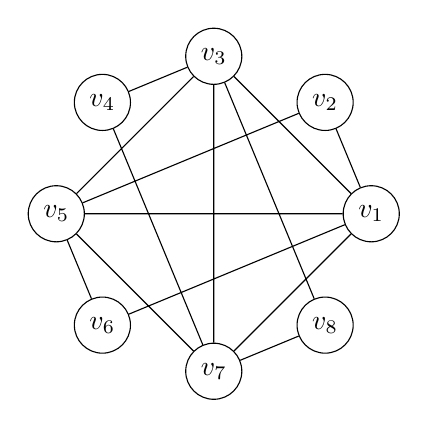
\begin{tikzpicture}[scale=2, bend angle=22.5]
\tikzstyle{every node}=[draw,shape=circle];
\foreach \i in {1,...,8}
{
\path (45*\i-45:1cm) node (v\i) {$v_\i$};
}
\draw
(v1) -- (v2) (v3) -- (v4) (v5) -- (v6) (v7) -- (v8)
(v1) -- (v3) (v3) -- (v5) (v5) -- (v7) (v7) -- (v1)
(v2) -- (v5) (v4) -- (v7) (v6) -- (v1) (v8) -- (v3)
(v1) -- (v5) (v3) -- (v7);
\end{tikzpicture}
		\end{example}
	\end{minipage}
	\hfill
	\begin{minipage}{0.5\linewidth}
%		\samplecommand{usepackage}\{tikz\}\\
%		\lstinputlisting{tikz/relation.tex}
	\end{minipage}
\end{frame}

\begin{frame}
	\begin{minipage}{0.53\linewidth}
		\begin{example}
			\centering
%			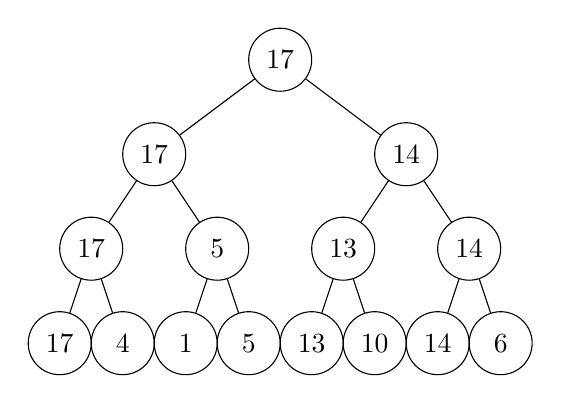
\begin{tikzpicture}[scale=0.8]
\tikzstyle{every node}=[draw,shape=circle,minimum size=0.8cm];
\node {17}[sibling distance=4cm]
child { node {17}[sibling distance=2cm]
	child {
		node {17}[sibling distance=1cm]
		child { node {17} }
		child { node {4} }
	}
	child {
		node {5}[sibling distance=1cm]
		child { node {1} }
		child { node {5} }
	}
}
child { node {14}[sibling distance=2cm]
	child {
		node {13}[sibling distance=1cm]
		child { node {13} }
		child { node {10} }
	}
	child {
		node {14}[sibling distance=1cm]
		child { node {14} }
		child { node {6} }
	}
};
\end{tikzpicture}
		\end{example}`
	\end{minipage}
	\hfill
	\begin{minipage}{0.42\linewidth}
%		\lstinputlisting{tikz/binary_tree.tex}
	\end{minipage}
\end{frame}